% PyStarLight: how a light curve is measured and timed (the method slides on their own).
% Build: make   (latexmk -pdf)   The same slides are part of the author's PySyzygos/PyStarLight talk.
\documentclass[aspectratio=169,11pt]{beamer}
% PyStarLight method slides: preamble (theme, colors, macros). Kept equal to PySyzygos' docs/math/preamble.tex,
% so the slides look the same in pystarlight_math.pdf and in the author's combined talk (which uses that one).
% Vectors after ISO 80000-2 (bold italic, half arrow); math slides carry an ID (\slideid) and numbered formulas
% (\tag / \eqtag, <ID>.<n>) that the code cites as "# Math: <ID>.<n>" (check_xref.py keeps both in step).
\usetheme[progressbar=frametitle, numbering=fraction, block=fill]{metropolis}
\usepackage[T1]{fontenc}
\usepackage[utf8]{inputenc}
\usepackage{graphicx}
\usepackage{booktabs,array}
\usepackage{siunitx}
\usepackage{amsmath,amssymb,bm}
% vectors after ISO 80000-2: bold italic with a half arrow (harpoon) over it; unit vectors with a hat
\newcommand{\vv}[1]{\overset{\rightharpoonup}{\bm{#1}}}
\newcommand{\uv}[1]{\hat{\bm{#1}}}
\newcommand{\pv}[1]{{\color{syzaccent}\vv{#1}}}   % a vector in the fundamental plane (2-D, from the observer): orange
% math slides: a short ID in a box at the right of the title bar; formulas numbered <ID>.<n> (\tag in displays,
% \eqtag at the end of a text line).
\newcommand{\slideid}[1]{\begin{tikzpicture}[remember picture, overlay]
  \node[anchor=east, draw=white, line width=0.6pt, rounded corners=2pt, inner sep=2.5pt, text=white,
        font=\footnotesize\bfseries] at ([xshift=-3mm, yshift=-0.55cm]current page.north east) {#1};
  \end{tikzpicture}\ignorespaces}
% less space above and below displayed formulas (after a font size command, which sets them): dense slides
\newcommand{\tightdisplays}{\setlength{\abovedisplayskip}{2pt}\setlength{\belowdisplayskip}{2pt}%
  \setlength{\abovedisplayshortskip}{0pt}\setlength{\belowdisplayshortskip}{2pt}}
\newcommand{\eqtag}[1]{\hfill{\scriptsize\textcolor{syzblue}{(#1)}}}
\newcommand{\grp}[1]{\multicolumn{2}{@{}l}{\footnotesize\textbf{#1}} \\}   % group heading row (conventions table)
% which library computes a step (tags on the astrometry and solver slides)
\newcommand{\libtag}[2]{{\setlength{\fboxsep}{1.2pt}\colorbox{#1!18}{\textcolor{#1!70!black}{\tiny\textsf{#2}}}}}
\newcommand{\SP}{\libtag{blue}{SpiceyPy}}
\newcommand{\AP}{\libtag{green}{astropy/ERFA}}
\newcommand{\SC}{\libtag{orange}{SciPy}}
\newcommand{\OWN}{\libtag{gray}{own code}}
\usepackage{hyperref}
\usepackage{fontawesome5}
\usepackage{multicol}
\usepackage{appendixnumberbeamer}
\usepackage{tikz}
\usetikzlibrary{positioning,arrows.meta,fit}
\usepackage{tcolorbox}\tcbuselibrary{theorems,skins}
% the numbered (key) formulas: each in a pale blue box (\tcbhighmath around the formula, the tag outside it)
\tcbset{highlight math style={enhanced, colback=syzblue!6, colframe=syzblue!40, boxrule=0.4pt, arc=2pt,
  left=3pt, right=3pt, top=0.5pt, bottom=0.5pt}}

% colors (close to the GUI's)
\definecolor{syzblue}{HTML}{1E3A5F}
\definecolor{syzaccent}{HTML}{D97706}
\setbeamercolor{frametitle}{bg=syzblue, fg=white}
\setbeamercolor{progress bar}{fg=syzaccent, bg=syzblue!20}
\setbeamercolor{title separator}{fg=syzaccent}
\setbeamercolor{alerted text}{fg=syzaccent}


% section page: metropolis' progressbar template plus the section's own subsections (from the table of contents,
% so they always match the outline), styled like the outline's subsection entries; \sectionlogo (empty unless
% set right before a \section) puts an image to the right of the title
\providecommand{\sectionlogo}{}
\makeatletter
\setbeamertemplate{section page}{%
  \centering
  \begin{minipage}{22em}
    \raggedright
    \usebeamercolor[fg]{section title}\usebeamerfont{section title}%
    \insertsectionhead\\[-1ex]
    \usebeamertemplate*{progress bar in section page}
    \par\vspace*{0.8ex}
    {\usebeamercolor[fg]{subsection title}\usebeamerfont{subsection title}%
     \setbeamertemplate{subsection in toc}{{\color{syzblue}\scriptsize$\blacktriangleright$}~\inserttocsubsection\par
       \vspace*{0.5ex}}%
     \tableofcontents[currentsection, sectionstyle=hide/hide, subsectionstyle=show/show/hide]}
  \end{minipage}%
  \ifx\sectionlogo\empty\else\hspace{1.5em}\begin{minipage}{6em}\sectionlogo\end{minipage}\fi
  \par
  \vspace{\baselineskip}
}
\makeatother

\graphicspath{{figures/}{../../src/pystarlight/}}

\title{PyStarLight: how a light curve is measured and timed}
\subtitle{Alignment, astrometry, photometry on the G scale, optimal extraction, step fit}
\InputIfFileExists{version.tex}{}{\newcommand{\pyversion}{?}}  % make writes it from src/pystarlight/__init__.py
\author{Percy Zahl}
\institute{\faGithub\ \href{https://github.com/pyzahl/PyStarLight}{github.com/pyzahl/PyStarLight}\\[0.3ex]
  For PyStarLight version \pyversion}
\date{\today}
\titlegraphic{\vspace*{-0.8cm}\hfill
\includegraphics[height=1.3cm]{pystarlight_logo.png}}

\begin{document}
\maketitle

\section{How it works}
% PyStarLight: how it works (the method slides, single source). Built on their own by pystarlight_math.tex
% (make), and \input by the author's private PySyzygos talk. Formulas follow the code (src/pystarlight):
% globaltrack.py (alignment, optimal extraction), wcs/reduce.py (astrometry, G zero point),
% normalize.py (ensemble magnitudes), steps.py (step fit).

% compact lists for these slides
\providecommand{\tightlist}{}\renewenvironment{tightlist}{\begin{itemize}\setlength{\itemsep}{0.1ex}\setlength{\topsep}{0.1ex}\setlength{\parsep}{0pt}}{\end{itemize}}
\providecommand{\sub}[1]{\par\noindent\hangindent=1.6em\hangafter=1\hspace*{0.8em}\textcolor{syzaccent}{\textendash}\ #1}   % a sub-point on its own line
\providecommand{\tightenum}{}\renewenvironment{tightenum}{\begin{enumerate}\setlength{\itemsep}{0.25ex}\setlength{\topsep}{0.1ex}\setlength{\parsep}{0pt}}{\end{enumerate}}

% ------------------------------------------------------------------------------------------------- overview
\begin{frame}{PyStarLight inside: from frames to D and R}
  \tightdisplays
  \centering
  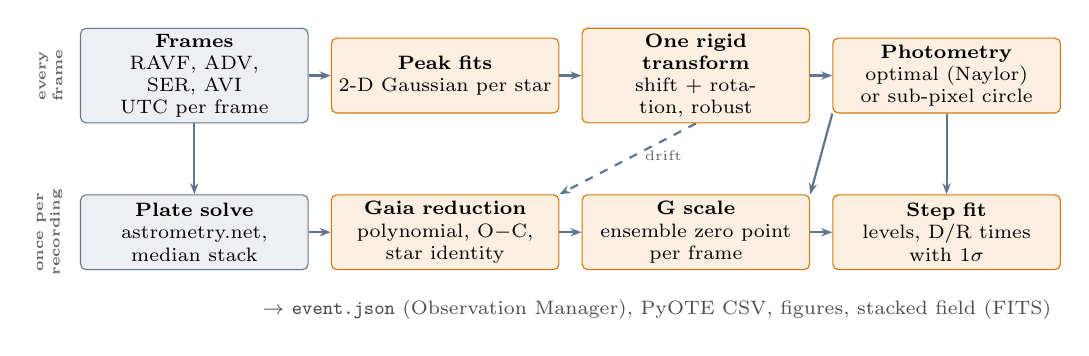
\begin{tikzpicture}[font=\scriptsize, node distance=0.9cm and 0.28cm,
      box/.style={draw=syzblue!70, fill=syzblue!8, rounded corners=2pt, align=center, minimum height=0.95cm,
                  text width=2.75cm, inner sep=2pt},
      acc/.style={box, draw=syzaccent, fill=syzaccent!12},
      arr/.style={-{Stealth[length=4pt]}, thick, syzblue!70}]
    % row 1: every frame
    \node[box] (mov) {\textbf{Frames}\\ RAVF, ADV, SER, AVI\\ UTC per frame};
    \node[acc, right=of mov] (fit) {\textbf{Peak fits}\\ 2-D Gaussian per star};
    \node[acc, right=of fit] (rig) {\textbf{One rigid transform}\\ shift + rotation, robust};
    \node[acc, right=of rig] (pho) {\textbf{Photometry}\\ optimal (Naylor)\\ or sub-pixel circle};
    % row 2: once per recording
    \node[box, below=of mov] (sol) {\textbf{Plate solve}\\ astrometry.net,\\ median stack};
    \node[acc, right=of sol] (red) {\textbf{Gaia reduction}\\ polynomial, O$-$C,\\ star identity};
    \node[acc, right=of red] (mag) {\textbf{G scale}\\ ensemble zero point\\ per frame};
    \node[acc, right=of mag] (stp) {\textbf{Step fit}\\ levels, D/R times\\ with $1\sigma$};
    \draw[arr] (mov) -- (fit);  \draw[arr] (fit) -- (rig);  \draw[arr] (rig) -- (pho);
    \draw[arr] (mov) -- (sol);  \draw[arr] (sol) -- (red);  \draw[arr] (red) -- (mag);  \draw[arr] (mag) -- (stp);
    \draw[arr] (pho) -- (stp);
    \draw[arr] (pho.south west) -- (mag.north east);
    \draw[arr, dashed] (rig.south) -- node[right, text=black!60, font=\tiny, pos=0.45] {drift} (red.north east);
    \node[rotate=90, anchor=south, text=black!60, font=\tiny, align=center] at ([xshift=-1mm]mov.west) {\textbf{every}\\\textbf{frame}};
    \node[rotate=90, anchor=south, text=black!60, font=\tiny, align=center] at ([xshift=-1mm]sol.west) {\textbf{once per}\\\textbf{recording}};
    \node[text=black!70, font=\scriptsize, below=0.25cm of stp.south east, anchor=north east]
      {$\to$ \texttt{event.json} (Observation Manager), PyOTE CSV, figures, stacked field (FITS)};
  \end{tikzpicture}\\[1ex]
  \raggedright\footnotesize
  \begin{tightlist}
    \item \textcolor{syzaccent}{\textbf{Orange}}: new code; \emph{PyMovie mode} stays (bit for bit), these slides
          show the \emph{global mode}
    \item \textbf{O$-$C}: observed minus calculated (measured position minus Gaia position)
    \item \textbf{D}, \textbf{R}: disappearance, reappearance of the star
  \end{tightlist}
\end{frame}

% ------------------------------------------------------------------------------------------------- alignment
\begin{frame}{Alignment: one transform carries every aperture}
  \tightdisplays
  \begin{columns}[T]
  \begin{column}{0.36\textwidth}
    \centering
    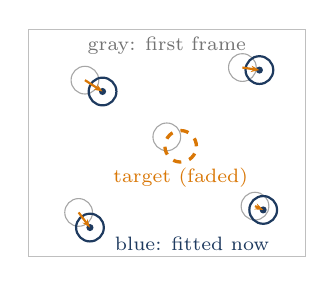
\begin{tikzpicture}[font=\scriptsize, scale=0.8]
      \draw[black!25] (0,0) rectangle (4.4,3.6);
      % reference positions (first frame) and the same stars now (shifted + rotated)
      \foreach \x/\y in {0.9/2.8, 3.4/3.0, 3.6/0.8, 0.8/0.7, 2.2/1.9}
        \draw[black!35] (\x,\y) circle (0.22);
      \foreach \x/\y in {1.18/2.62, 3.67/2.96, 3.73/0.74, 0.98/0.46} {
        \fill[syzblue] (\x,\y) circle (1.6pt);
        \draw[syzblue, thick] (\x,\y) circle (0.22);
      }
      \foreach \a/\b/\c/\d in {0.9/2.8/1.18/2.62, 3.4/3.0/3.67/2.96, 3.6/0.8/3.73/0.74, 0.8/0.7/0.98/0.46}
        \draw[-{Stealth[length=3pt]}, syzaccent, thick] (\a,\b) -- (\c,\d);
      % the target: faded, placed by the others
      \draw[syzaccent, very thick, dashed] (2.42,1.75) circle (0.25);
      \node[syzaccent] at (2.42,1.25) {target (faded)};
      \node[black!55] at (2.2,3.35) {gray: first frame};
      \node[syzblue] at (2.6,0.2) {blue: fitted now};
    \end{tikzpicture}\\[0.5ex]
    \raggedright\scriptsize
    \begin{tightlist}
      \item wind shake, drift, field rotation
      \item all stars move together
      \item a faded star is carried by the others
    \end{tightlist}
  \end{column}
  \begin{column}{0.62\textwidth}
    \scriptsize
    \begin{tightenum}
      \item \textbf{Peak fit} per star: $I = b + a\,e^{-r^2/2s^2}$
        \sub{kept if SNR $\ge 5$ and $0.5\,\bar s < s < 2\,\bar s$ (no cosmic rays)}
      \item \textbf{Weighted rigid fit} $\vv{p}_i \approx R(\theta)\,\vv{q}_i + \vv{d}$
        \[ \theta = \operatorname{atan2}\Big(\textstyle\sum w_i\, \vv{a}_i \times \vv{b}_i,\ \sum w_i\, \vv{a}_i\cdot\vv{b}_i\Big),
           \quad \vv{d} = \vv{c}_p - R(\theta)\,\vv{c}_q \]
        \sub{$w_i = \min(\mathrm{SNR}_i, 100)^2$}\sub{$\vv{a}_i, \vv{b}_i$: positions about the weighted centers $\vv{c}_q, \vv{c}_p$}\sub{start from the median shift, clip at $4\times$ robust residual}
      \item \textbf{Occultation aware}
        \sub{a star dimming $< 0.4\times$ the others' change leaves the fit}\sub{clouds dim all stars: no effect}
      \item \textbf{Target's own drift}: smoothed, interpolated across the event
    \end{tightenum}
  \end{column}
  \end{columns}
\end{frame}

% ------------------------------------------------------------------------------------------------- astrometry
\begin{frame}{Astrometry: a Gaia DR3 reduction, in the manner of PRAIA}
  \tightdisplays
  \begin{columns}[T]
  \begin{column}{0.56\textwidth}
    \footnotesize
    \begin{tightenum}
      \item \textbf{Match}: astrometry.net WCS pairs stars with local Gaia DR3 (proper motions to the date)
      \item \textbf{Tangent plane} at $(\alpha_0, \delta_0)$:
        \[ \xi = \frac{\cos\delta\,\sin\Delta\alpha}{D},\quad
           \eta = \frac{\sin\delta\cos\delta_0 - \cos\delta\sin\delta_0\cos\Delta\alpha}{D} \]
      \item \textbf{Plate model}, $u, v$ = normalized pixel position:
        \[ \xi = \textstyle\sum_{k+l \le n} a_{kl}\, u^k v^l,\quad \eta = \sum_{k+l \le n} b_{kl}\, u^k v^l \]
        \sub{$n = 1$--$3$, $\ge 3$ stars per parameter}\sub{else 4 constants (mirror image tested)}
      \item \textbf{Outliers}: dropped one by one while O$-$C $> 3\sigma$
    \end{tightenum}
  \end{column}
  \begin{column}{0.42\textwidth}
    \footnotesize
    \begin{tcolorbox}[colback=syzblue!5, colframe=syzblue!40, boxrule=0.4pt, arc=2pt, left=3pt, right=3pt]
      \textbf{What it gives}
      \begin{tightlist}
        \item O$-$C per star: \emph{measured} precision
        \item RA/Dec of any pixel, with error
        \item target vs its Gaia star: wrong or blended star flagged
        \item names: Gaia DR3, UCAC4, TYC
      \end{tightlist}
    \end{tcolorbox}
    \vspace{0.4ex}
    \scriptsize\textbf{ASTRID}, 2.07\,$''$/px:
    \begin{tightlist}
      \item residuals 0.85\,$''$ $\to$ \textbf{0.5\,$''$} ($\frac14$ px)
      \item 0.4\,$''$ offset removed
    \end{tightlist}
    {\tiny O$-$C: observed minus calculated (cf.\ slide CH)\par}
  \end{column}
  \end{columns}
\end{frame}

% ------------------------------------------------------------------------------------------------- G scale
\begin{frame}{Photometry on the Gaia G scale}
  \tightdisplays
  \footnotesize
  \begin{tightenum}
    \item \textbf{One frame}: zero point from the field
      \[ m_i = -2.5\log_{10} F_i + Z, \qquad Z = \operatorname{median}_i\big(G_i + 2.5\log_{10} F_i\big) \]
      \sub{circle $2\times$ FWHM, annulus background, $3\sigma$ clipping (variables, blends)}\sub{target's $m$ vs its $G$: identity check}
    \item \textbf{Light curve}: references form one \emph{ensemble star}
      \begin{tcolorbox}[colback=syzblue!6, colframe=syzblue!40, boxrule=0.4pt, arc=2pt, left=3pt, right=3pt, top=0pt, bottom=0pt]
      \[ m_\mathrm{ens} = -2.5\log_{10}\sum_{r} 10^{-0.4\,G_r}, \qquad
         m(t) = m_\mathrm{ens} - 2.5\log_{10}\frac{s(t)}{\tilde S(t)}, \quad \tilde S = \text{smoothed}\ \textstyle\sum_r s_r \]
      \end{tcolorbox}
      \sub{zero point per frame: clouds, extinction drop out}\sub{$s/\tilde S$ = linear flux for the step fit}
    \item \textbf{Levels}: $m$ with error $1.0857\,\sigma_{\bar f}/\bar f$; near zero flux: ``fainter than'' $3\sigma$
  \end{tightenum}
  \vspace{0.6ex}
  {\scriptsize\textbf{Limits}: scatter $\sim$0.2\,mag is mostly color (sensor band $\ne$ G); saturated references left out, never repaired.\par}
\end{frame}

% ------------------------------------------------------------------------------------------------- Naylor
\begin{frame}{Optimal extraction (Naylor 1998): weight the pixels by the star}
  \tightdisplays
  \begin{columns}[T]
  \begin{column}{0.54\textwidth}
    \scriptsize
    \begin{tightlist}
      \item $P_j$: star profile in pixel $j$ (Gaussian of the seeing, unit flux)
      \item $D_j$: data minus background
      \item $\sigma_b$: background noise per pixel
    \end{tightlist}
    \begin{tcolorbox}[colback=syzblue!6, colframe=syzblue!40, boxrule=0.4pt, arc=2pt, left=3pt, right=3pt, top=0pt, bottom=0pt]
    \[ \hat F = \sum_j W_j D_j,\qquad W_j = \frac{P_j}{\sum_k P_k^2} \]
    \end{tcolorbox}
    \begin{tightlist}
      \item \textbf{unbiased}: $\langle \hat F\rangle = F \sum_j W_j P_j = F$
      \item \textbf{linear}: deep drops stay exact
      \item \textbf{noise} (background-limited):
        \[ \sigma^2_\mathrm{opt} = \frac{\sigma_b^2}{\sum P_j^2} \quad\text{vs}\quad
           \sigma^2_\mathrm{circ} = \frac{N_\mathrm{pix}\,\sigma_b^2}{f_\mathrm{enc}^2} \]
      \item \textbf{optimal}: $W \propto P$ minimizes $\sum W^2$ (Cauchy--Schwarz)
      \item same $P$ for all stars: profile errors cancel
    \end{tightlist}
  \end{column}
  \begin{column}{0.44\textwidth}
    \footnotesize
    \textbf{SNR gain} (sky-limited, Gaussian PSF):\\[0.4ex]
    \centering
    \begin{tabular}{@{}lccc@{}}
      \toprule
      FWHM (px) & 2.4 & 3.5 & 4.7 \\
      \midrule
      vs circle $1.5\times$FWHM & 1.65 & 1.75 & 1.71 \\
      vs best circle ($\approx 0.63\times$) & 1.08 & 1.10 & 1.11 \\
      \bottomrule
    \end{tabular}\\[0.3ex]
    {\scriptsize (computed: $\sqrt{\sum P^2}$ vs $f_\mathrm{enc}/\sqrt{N_\mathrm{pix}}$)\par}
    \raggedright\vspace{0.8ex}
    \begin{tcolorbox}[colback=syzaccent!8, colframe=syzaccent!60, boxrule=0.4pt, arc=2pt, left=3pt, right=3pt]
      \scriptsize
      \textbf{Wins}:
      \begin{tightlist}
        \item faint stars
        \item sky, read-out, dark noise (per pixel)
      \end{tightlist}
      \textbf{Cannot help}:
      \begin{tightlist}
        \item scintillation (same factor in every pixel)
        \item bright, photon-limited stars
      \end{tightlist}
      Short exposures: compare both (\emph{Optimal} checkbox)
    \end{tcolorbox}
  \end{column}
  \end{columns}
\end{frame}

% ------------------------------------------------------------------------------------------------- step fit 1
\begin{frame}{Event timing, part 1: how many steps, and where}
  \tightdisplays
  \begin{columns}[T]
  \begin{column}{0.56\textwidth}
    \footnotesize
    \textbf{Model}: piecewise constant flux $y_t$, no event window to mark
    \begin{tightenum}
      \item \textbf{Noise} $\sigma$: robust rms of $y_{t+1} - y_t$, $/\sqrt 2$
      \item \textbf{Binary segmentation} (Olshen et al.\ 2004): a split gains
        \[ \Delta S = \frac{n_1 n_2}{n_1 + n_2}\,(\bar y_1 - \bar y_2)^2 \]
        \sub{kept while $\Delta S/\sigma^2 > 6 \ln n$ (BIC: $2\ln n$)}\sub{also a \emph{box}: short dip inside a segment}
      \item \textbf{Clean up}
        \sub{backward elimination, points re-placed}\sub{1--2 frame level between neighbours = partial frame}\sub{every step $\ge 5\sigma$}
    \end{tightenum}
  \end{column}
  \begin{column}{0.42\textwidth}
    \centering
    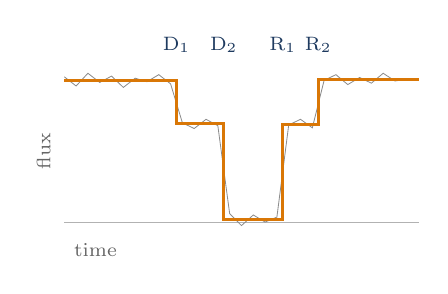
\begin{tikzpicture}[font=\scriptsize, xscale=0.75, yscale=0.9]
      % noisy curve with a two-step event, the fitted levels on top
      \draw[black!30] (0,0) -- (6,0);
      \draw[black!45, line width=0.3pt]
        plot coordinates {(0,2.05) (0.2,1.92) (0.4,2.1) (0.6,1.97) (0.8,2.06) (1.0,1.9) (1.2,2.03) (1.4,1.98)
        (1.6,2.08) (1.8,1.95) (2.0,1.4) (2.2,1.32) (2.4,1.45) (2.6,1.36) (2.8,0.12) (3.0,-0.05) (3.2,0.1)
        (3.4,0.0) (3.6,0.07) (3.8,1.37) (4.0,1.45) (4.2,1.33) (4.4,2.0) (4.6,2.08) (4.8,1.94) (5.0,2.04)
        (5.2,1.96) (5.4,2.1) (5.6,1.99) (5.8,2.02)};
      \draw[syzaccent, very thick] (0,2.0) -- (1.9,2.0) -- (1.9,1.39) -- (2.7,1.39) -- (2.7,0.04) -- (3.7,0.04)
        -- (3.7,1.38) -- (4.3,1.38) -- (4.3,2.01) -- (6,2.01);
      \foreach \x/\l in {1.9/D$_1$, 2.7/D$_2$, 3.7/R$_1$, 4.3/R$_2$}
        \node[syzblue] at (\x,2.5) {\l};
      \node[black!60, anchor=west] at (0,-0.4) {time};
      \node[black!60, rotate=90] at (-0.35,1.0) {flux};
    \end{tikzpicture}\\[0.6ex]
    \raggedright\scriptsize
    \begin{tightlist}
      \item pairs nested like brackets: D$_2$R$_1$ inner, D$_1$R$_2$ outer
      \item levels in mag, or ``fainter than''
    \end{tightlist}
    \vspace{0.4ex}
    \textbf{Tested}:
    \begin{tightlist}
      \item injected events found within $\sigma$
      \item rms of (fit$-$true)$/\sigma$: 0.85--1.25
      \item 200 noise-only curves: no step
    \end{tightlist}
  \end{column}
  \end{columns}
\end{frame}

% ------------------------------------------------------------------------------------------------- step fit 2
\begin{frame}{Event timing, part 2: the time to a fraction of a frame}
  \tightdisplays
  \begin{columns}[T]
  \begin{column}{0.46\textwidth}
    \centering
    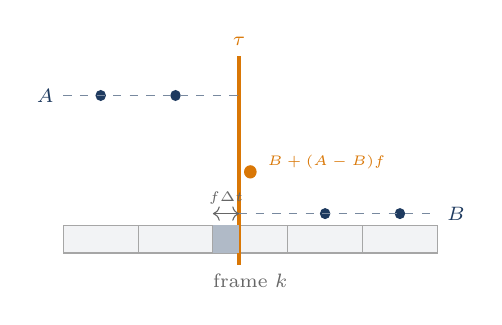
\begin{tikzpicture}[font=\scriptsize, xscale=0.95]
      % exposures as boxes; the step tau inside frame k
      \foreach \i in {0,...,4}
        \draw[black!35, fill=syzblue!6] (\i*1.0,0) rectangle ++(1.0,0.35);
      \draw[syzaccent, very thick] (2.35,-0.15) -- (2.35,2.5) node[above] {$\tau$};
      \fill[syzblue!35] (2.0,0) rectangle (2.35,0.35);
      \node[black!60] at (2.5,-0.35) {frame $k$};
      \draw[<->, black!60] (2.0,0.5) -- (2.35,0.5) node[midway, above, font=\tiny] {$f\Delta t$};
      % levels and the mixed frame
      \foreach \i/\y in {0/2.0, 1/2.0, 3/0.5, 4/0.5}
        \fill[syzblue] (\i*1.0+0.5,\y) circle (2pt);
      \fill[syzaccent] (2.5,1.03) circle (2.4pt);
      \draw[syzblue!60, dashed] (0,2.0) -- (2.35,2.0);  \draw[syzblue!60, dashed] (2.35,0.5) -- (5,0.5);
      \node[syzblue, anchor=east] at (0,2.0) {$A$};  \node[syzblue, anchor=west] at (5,0.5) {$B$};
      \node[syzaccent, anchor=west, font=\tiny] at (2.6,1.15) {$B + (A-B) f$};
    \end{tikzpicture}\\[0.5ex]
    \raggedright\scriptsize
    \begin{tightlist}
      \item frame = exposure $\Delta t$ at \emph{mid-exposure}
      \item stamps shifted as recorded: RAVF start, ADV middle
    \end{tightlist}
  \end{column}
  \begin{column}{0.52\textwidth}
    \footnotesize
    \begin{tightenum}
      \item \textbf{Partial frame}: mix of both levels by $f_t(\tau)$
        \[ \mu_t(\tau) = B + (A - B)\, f_t(\tau) \]
        \[ \chi^2(\tau) = \sum_t \frac{(y_t - \mu_t(\tau))^2}{f_t\sigma_A^2 + (1-f_t)\sigma_B^2} \]
      \item \textbf{Scan} $\tau$: $1/20$-frame grid, levels fixed
      \item \textbf{$1\sigma$} = the larger of
        \sub{half the $\chi^2_\mathrm{min} + 1$ interval}\sub{scatter in 300 simulated curves (catches a frame off)}
    \end{tightenum}
    \vspace{0.4ex}
    \scriptsize
    \begin{tightlist}
      \item Fringilla 2025: 4 contacts, $\sigma$ 0.025--0.034\,s
      \item not modelled: diffraction, star diameter, grazes
      \item for a report: compare with PyOTE
    \end{tightlist}
  \end{column}
  \end{columns}
\end{frame}


\begin{frame}{References}
  \footnotesize
  \begin{itemize}\setlength{\itemsep}{0.4ex}
    \item PyMovie and PyOTE: B.~Anderson, github.com/bob-anderson-ok
    \item Optimal extraction: Naylor (1998), MNRAS 296, 339
    \item PRAIA: Assafin et al.\ (2011), Gaia-FUN-SSO workshop proceedings, IMCCE, p.\,85
    \item Astrometry.net: Lang et al.\ (2010), AJ 139, 1782
    \item Change points: Olshen et al.\ (2004), Biostatistics 5, 557
    \item Gaia DR3: Gaia Collaboration, Vallenari et al.\ (2023), A\&A 674, A1
  \end{itemize}
\end{frame}
\end{document}
